

Mithilfe von Scopes oder Plots werden nun die gesuchten Signale abgegriffen und als Funktionen der Zeit dargestellt. \\
Die Abbildungen \ref{fig:Moment}, \ref{fig:Omega} und \ref{fig:StreckeundUnwuchtkraft} sind Plots aus Matlab, die wie folgt definiert wurden:

\begin{figure}[hbt]
	\centering
	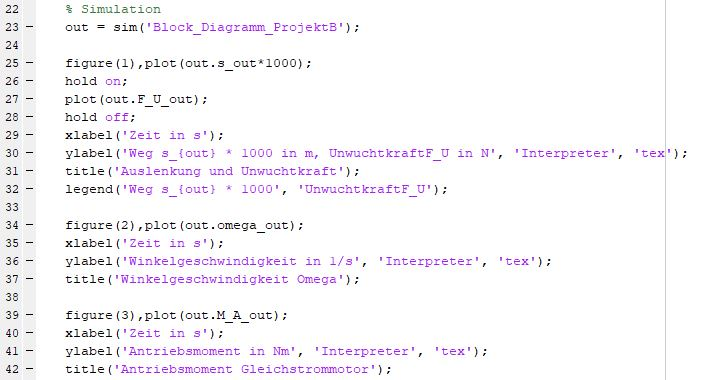
\includegraphics[width=1\linewidth]{Images/Simulationscode}
	\caption{}
	\label{fig:Simcode}
\end{figure}

In den folgenden Abbildungen \ref{fig:Moment}, \ref{fig:Omega} und \ref{fig:StreckeundUnwuchtkraft} sind das Motormoment $M$, die Winkelgeschwindigkeit $\Omega$, die Strecke $s$ und die Unwuchtkraft $F_U$ über die Zeit von $100 \milli\second$ dargestellt. Für kleine Änderungen der Dämpfungskonstanten können die translatorischen und rotatorischen Bewegungsgleichungen getrennt betrachtet werden.

\begin{figure}[hbt]
	\centering
	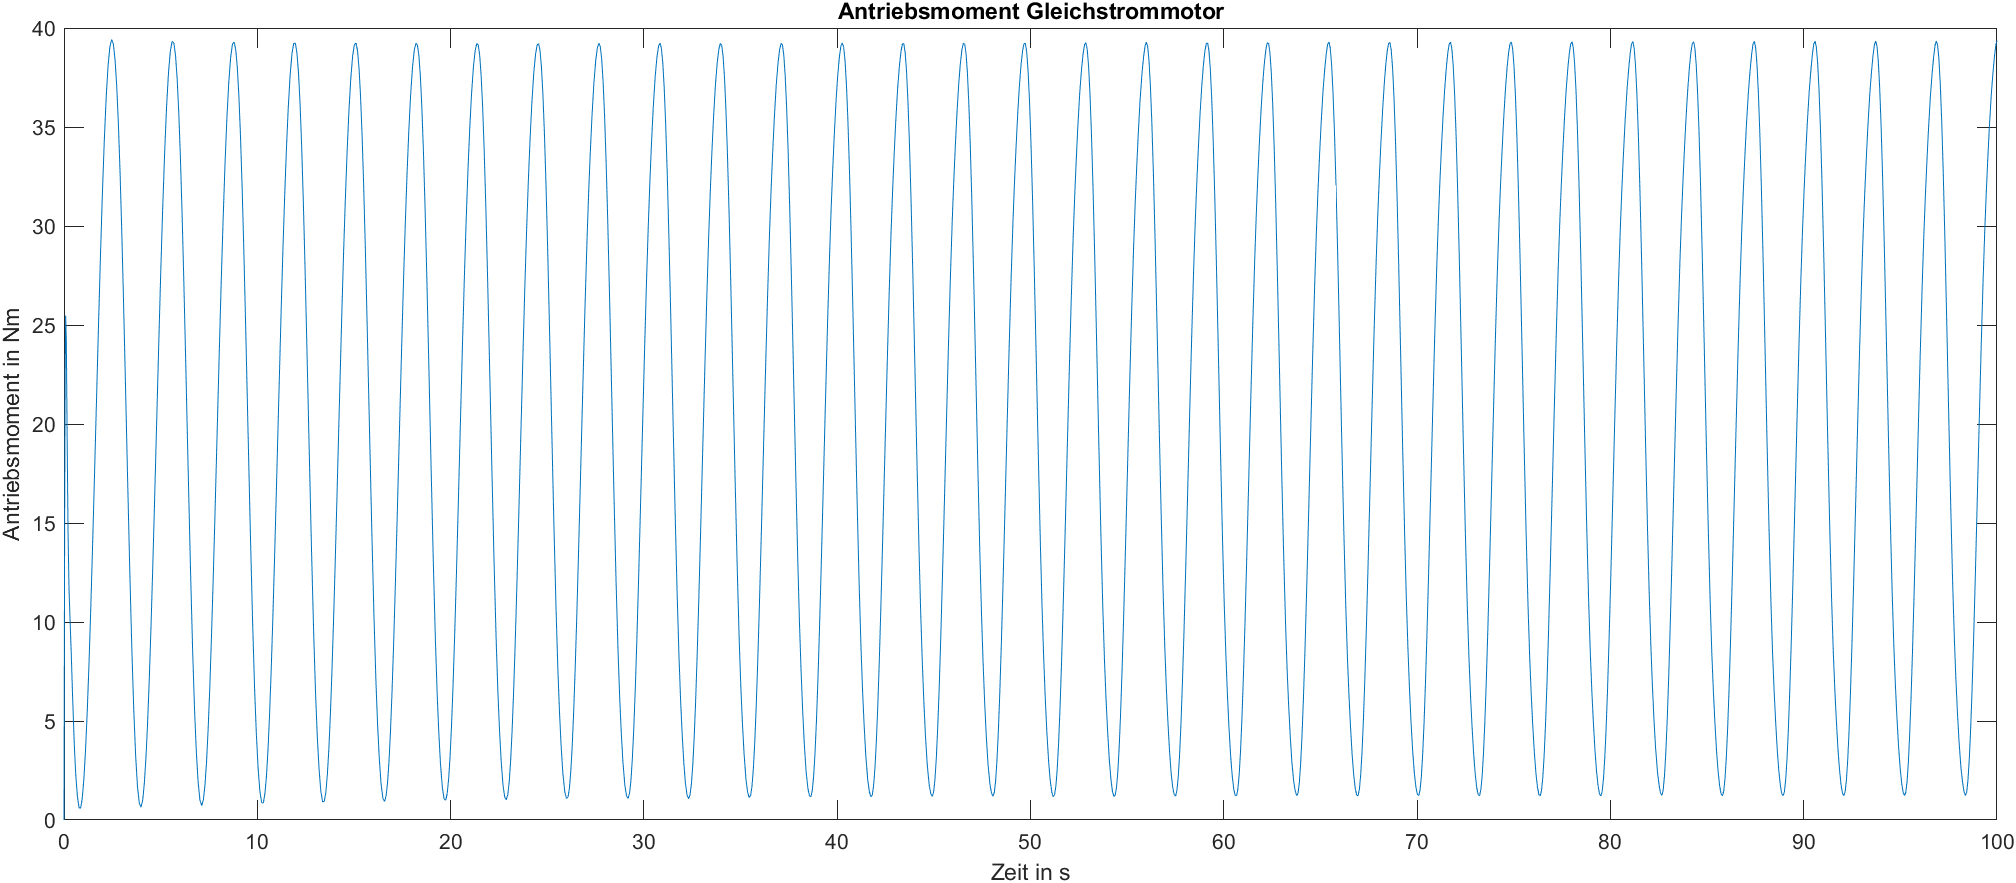
\includegraphics[width=1\linewidth]{Images/Moment}
	\caption{Simulationsergebnis: Antriebsmoment des Gleichstrommotors}
	\label{fig:Moment}
\end{figure}

Das in \ref{fig:Moment} dargestellte Antriebsmoment ist hauptsächlich abhängig von der rotatorischen Bewegungsgleichung des Schwingsystems, ebenso wie die Winkelgeschwindigkeit $\Omega$. Im Verlauf dieser beiden Größen und aus dem gegeben Parametersatz kann dieses Teilsystem dem Schwingungsfall zugewiesen werden, dessen zeitlicher Verlauf auf eine ungedämpfte Schwingung deuten lässt und damit auch auf die Grenzstabilität des Systems. Zur genaueren Analyse, wird der Wert der rotatorischen Dämpfungskonstante $d_r$ verändert, um die Abhängigkeit von dieser zu überprüfen. 
Verdoppelt man den Wert von $d_r$ verschiebt sich die Amplitude des Antriebsmoments um 20Nm nach oben. Bei einer weiteren Erhöhung wird die Kurve ebenfalls immer weiter nach oben gerückt, wobei sich jedoch die Amplitude von 40Nm kaum verändert. 

\begin{figure}[hbt]
	\centering
	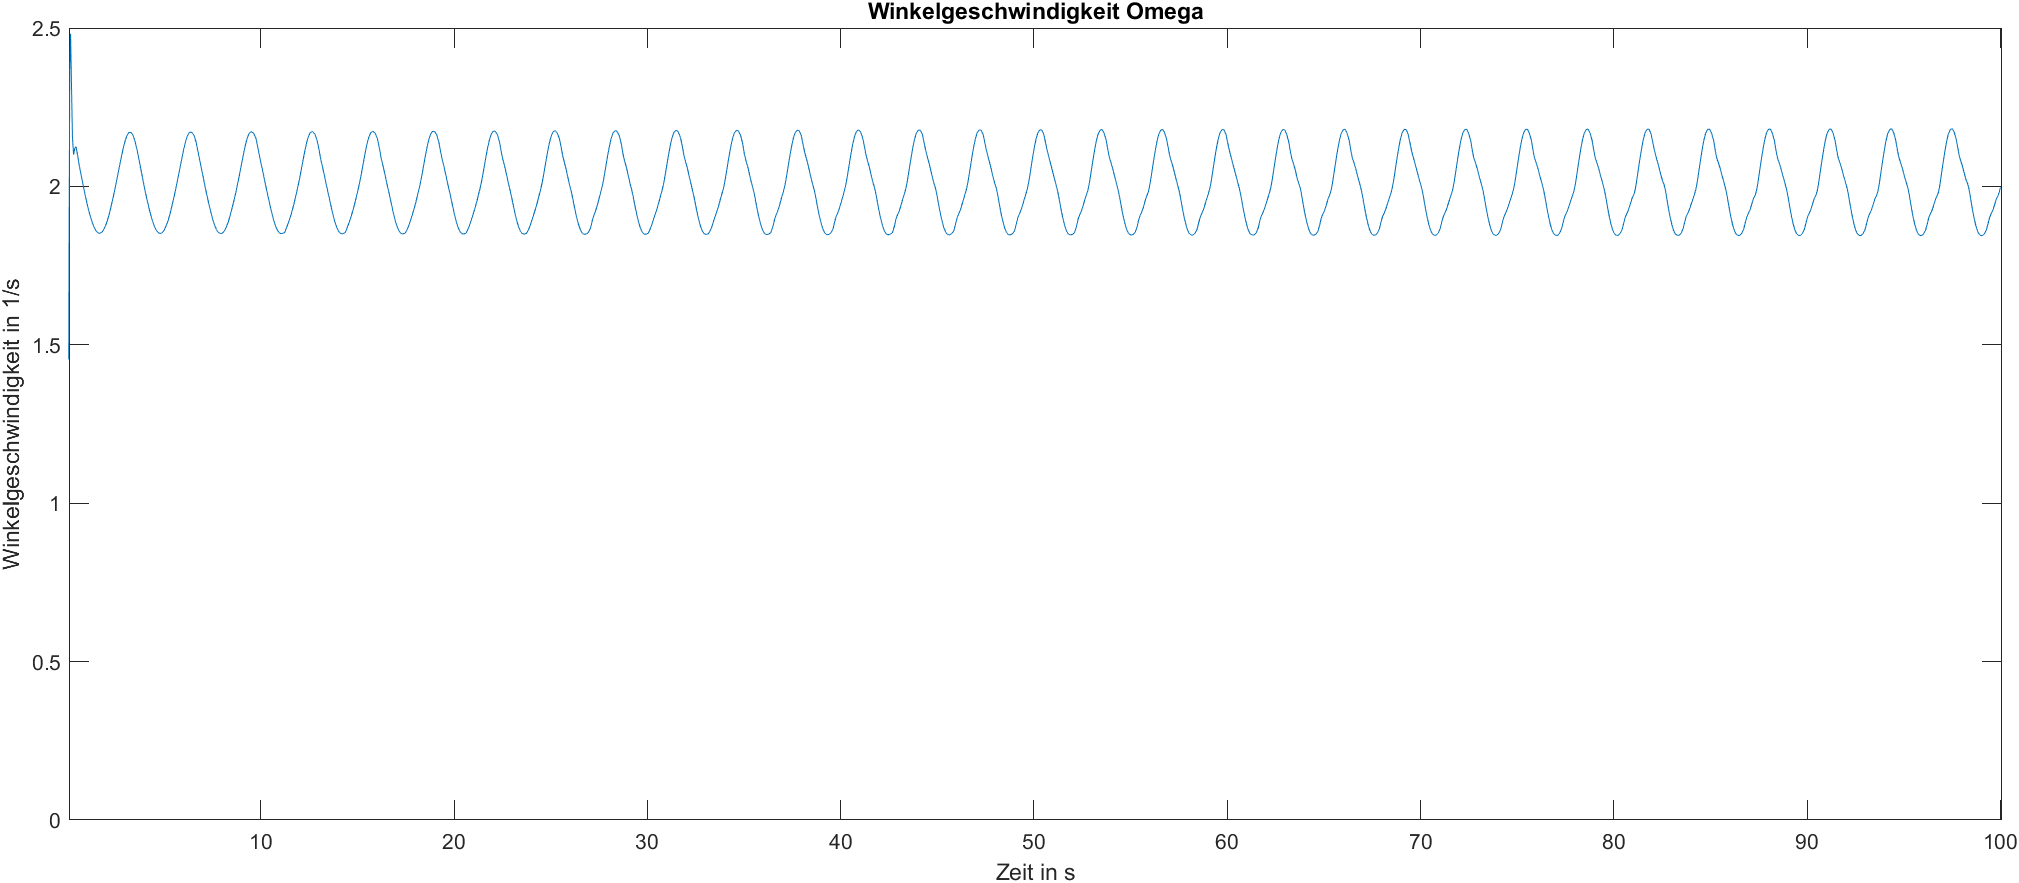
\includegraphics[width=1\linewidth]{Images/Omega}
	\caption{Simulationsergebnis: Winkelgeschwindigkeit des mechatronischen Systems}
	\label{fig:Omega}
\end{figure}

Die Veränderungen an der Dämpfungskonstante hatten keinen nennenswerten Einfluss auf die Winkelgeschwindigkeit. Um diese marginal zu Beeinflussen müsste die Motorkonstante $K_A$ angepasst werden, was sich wiederum auf das Antriebsmoment und die Unwuchtkraft auswirkt.

Auffällig ist in Abbildung \ref{fig:StreckeundUnwuchtkraft}, dass die Auslenkung die doppelte Frequenz der Unwuchtkraft hat.

\begin{figure}[hbt]
	\centering
	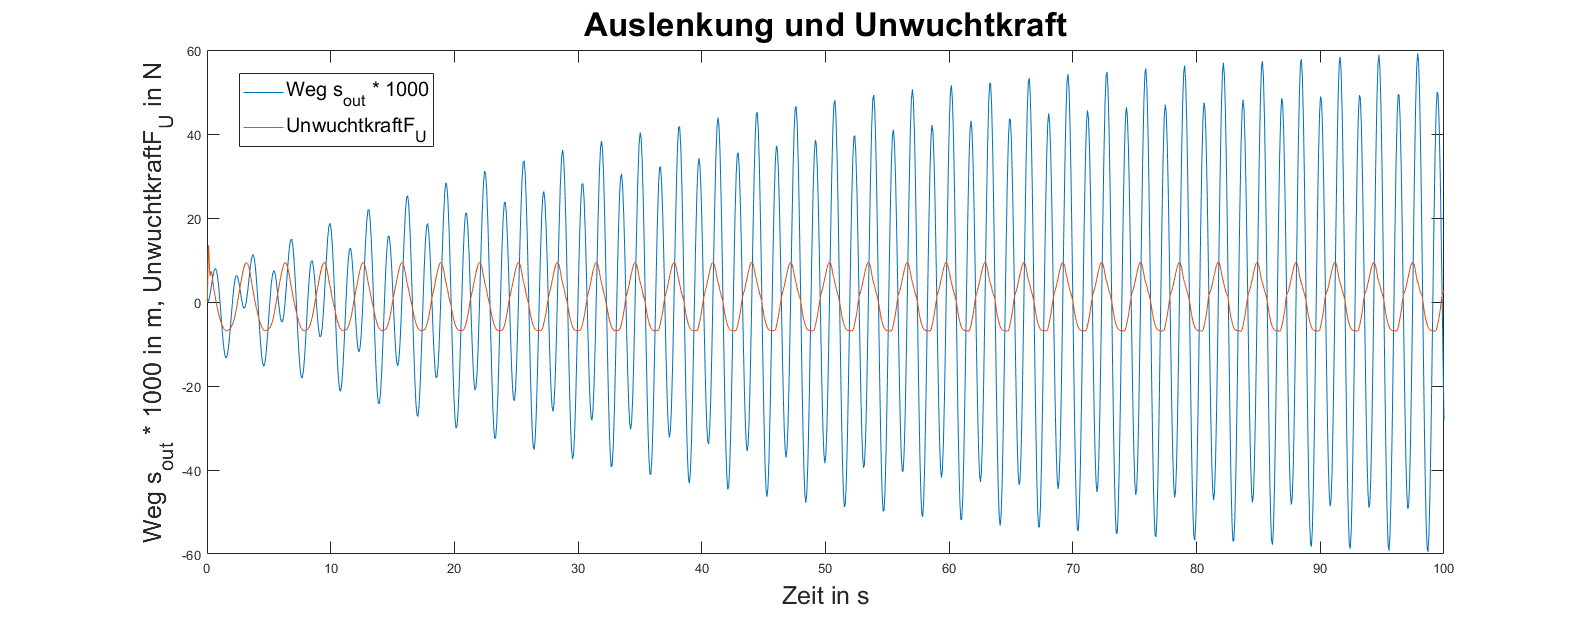
\includegraphics[width=1\linewidth]{Images/StreckeundUnwuchtkraft}
	\caption{Simulationsergebnis: Auslenkung$\cdot$1000 und Unwuchtkraft des mechatronischen Systems}
	\label{fig:StreckeundUnwuchtkraft}
\end{figure}



